%Modelování a simulace
%Filip Čižmár (xcizma06), Samuel Križan (xkriza06)
%2020

\documentclass[11pt,a4paper,titlepage]{article}
\usepackage[left=2cm,text={17cm,24cm},top=3cm]{geometry}
\usepackage[T1]{fontenc}
\usepackage[czech]{babel}
\usepackage[utf8]{inputenc}
\bibliographystyle{czplain}
\usepackage{times}
\usepackage{graphicx}

\graphicspath{{.}}

\begin{document}

\begin{titlepage}
\begin{center}
    {\textsc{\Huge Vysoké učení technické v~Brně}}\\
    \smallskip
    {\huge\textsc{Fakulta informačních technologií}}\\
    \bigskip
    \vspace{\stretch{0.382}}    
    \LARGE{Modelování a simulace\,--\,projekt}\\
    \smallskip
    \Huge{Téma č. 1: Epidemiologické modely pomocí celulárních automatů}\\
    \vspace{\stretch{0.618}}
\end{center}
    { 6. 12. 2020 \hfill Filip Čižmár (xcizma06), Samuel Križan (xkriza06) }
\end{titlepage}


\setlength{\parskip}{0pt}
\tableofcontents
\setlength{\parskip}{0pt}

\newpage


\section{Úvod}
Tento projekt a inžinierska správa sa zaoberajú problematikou šírenia epidémie vírusu. Pri tvorbe modelu boli využité verejno-dostupné dáta a štatistiky pandémie Covid-19, ktorými bol model následne naplnený. Teda výsledok je prispôsobený a zameraný na vírus Covid-19, ale model by mal byť využiteľný aj pri iných epidémiach.
Cieľom modelu je štatisticky znázorniť priebeh šírenia vírusu Covid-19 a potvrdiť / vyvrátiť účinnosť jednotlivých opatrení zavedených na spomalenie šírenia vírusu.


\subsection{Autori a zdroje}
Autormi modelu sú Filip Čižmár (xcizma06) a Samuel Križan (xkriza06). Zadanie práce spadá pod Vysoké učení technické v Brně, projekt predmetu Modelování a simulace. Presné zadanie je Téma č. 1: Epidemiologické modely pomocí celulárních automatů. \cite{Zadanie}

Štatistické informácie boli prevzaté z článkov štúdií verejne dostupných na internete, a kde zdroj je jednoznačný, budú vždy označené patričnými informáciami v poslednej sekcii dokumentu - Referencie.

Koncept a matematický základ modelu bol prevzatý z článku Using Cellular Automata to Simulate Epidemic Diseases\cite{Zdroj}.

\subsection{Validita modelu}
Validita modelu bola overená porovnaním reálnych štatistík priebehu covid-19 s výstupmi modelu. 

\section{Rozbor témy a použitých metód/technológií}
Informácie týkajúce sa implementácie modelu boli získané z článku vedeckého časopisu Applied Mathematical Sciences - Using Cellular Automata to Simulate Epidemic Diseases.\cite{Zdroj}
Článok popisuje princíp využitia celulárnych automatov na modelovanie šírenia epidémií. Celulárne automaty sú implementačne jednoduché dvojrozmerné modely schopné simulovať komplexné biologické či environmentálne javy z reálneho života, a preto sú vhodné aj na modelovanie problematiky epidémií.

\subsection{Použité postupy}
Celulárny automat tohto projektu vychádza z matematického modelu SIR - Susceptible (náchylní), Infected (infikovaní), Recovered (uzdravení). Rovnako ako vo vyššie zmienenom článku bola použitá možnosť Moorovho okolia bunky - teda všetky bunky v 3x3 štvorci so stredom v aktuálnej bunke.

\noindent Jazyk implementácie je C++. Žiadne vonkajšie knižnice neboli použité.

\subsection{Pôvod použitých metód}
Všetky použité metódy sú prebrané z nasledovného článku:

\noindent https://www.researchgate.net/publication/228819056\_Using\_Cellular\_Automata\_to\_Simulate\_Epidemic\_Diseases

\section{Podstata simulačných experimentov a ich priebeh}
Podstatou experimentov bolo potvrdiť validitu modelu voči verejne-dostupným štatistikám z prvej/druhej vlny koronavírusu a následne zistiť efektivitu jednotlivých opatrení na spomalenie šírenia vírusov.

\subsection{Postup experimentovania}
Všetky experimenty prebiehali mapovaním výstupu modelu do grafov v programe GNU Octave, kde osa x reprezentuje po sebe nasledujúce dni a osa y reprezentuje celkové percento (resp. pomer) nakazených. Vstupné konštanty (koeficient pohybu obyvateľov, koeficient prenosu a pod.) boli pred štartom programu vždy zmenené, program bol viackrát spustený s rôznymi hodnotami a jednotlivé výstupy boli následne porovnané s reálnymi hodnotami.

\subsection{Jednotlivé experimenty}
\subsubsection{Experiment č. 1}
Prvý experiment popisuje šírenie vírusu pri zmene koeficientu pohybu. Štatistiky z reálneho sveta hovoria, že pri obmedzení pohybu obyvateľov štátu sa šírenie vírusu spomalí a maximálne množstvo súčasne nakazených obyvateľov sa zníži, brániac tak preplneniu zdravotníckych zariadení.

Pri experimente boli použité hodnoty koeficientu pohybu 15, 3.5 a 0. Tieto čísla popisujú počet náhodných stretnutí s bunkami mimo Moorovho okolia bunky, kde 15 reprezentuje neobmedzený pohyb, 3.5 pohyb mierne obmedzený a 0 reprezentuje zákaz pohybu na väčšie vzdialenosti. Obyvatelia sa teda pohybujú len v rámci Moorovho okolia ich bunky.

\begin{figure}[h!]
    \center
    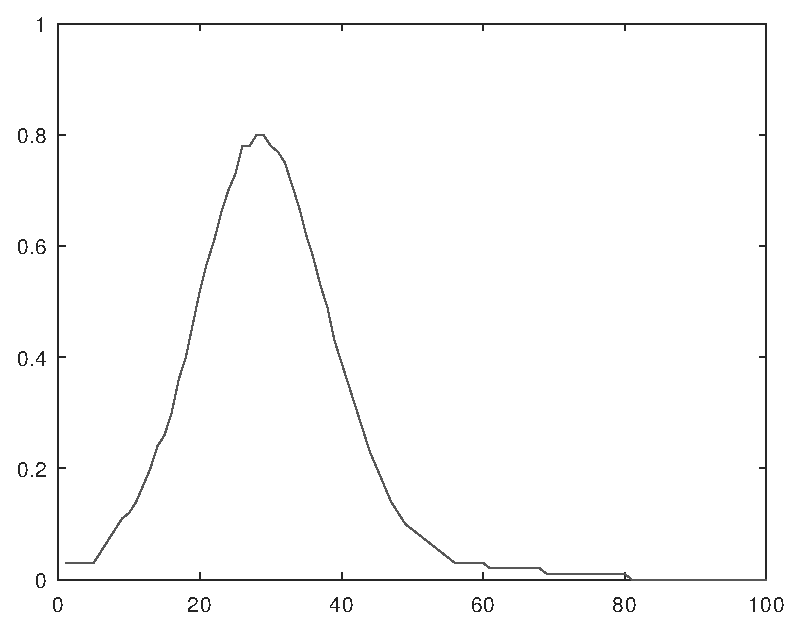
\includegraphics[width=.39\linewidth]{movement-rate-15.eps}
    \caption{Koeficient pohybu 15}
\end{figure}

\begin{figure}[h!]
    \center
    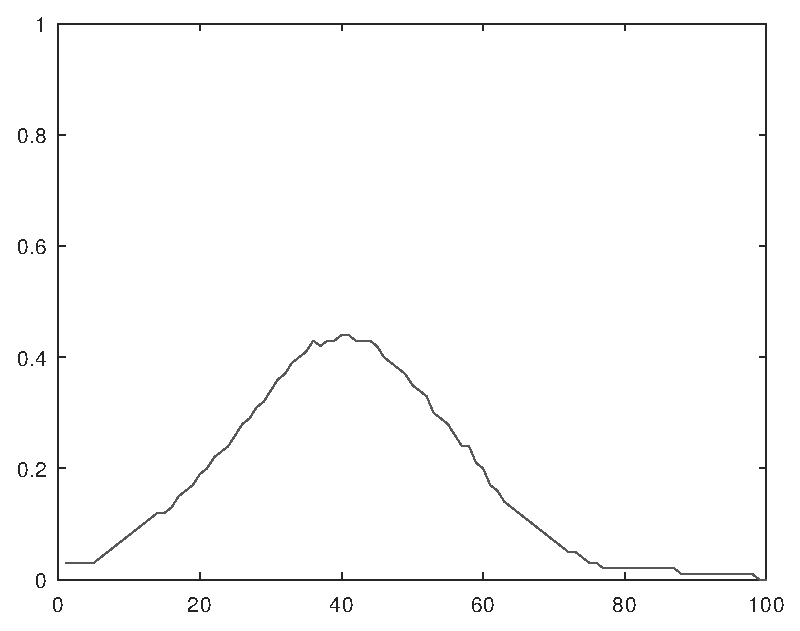
\includegraphics[width=.39\linewidth]{movement-rate-3_5.eps}
    \caption{Koeficient pohybu 3.5}
\end{figure}

\begin{figure}[h!]
    \center
    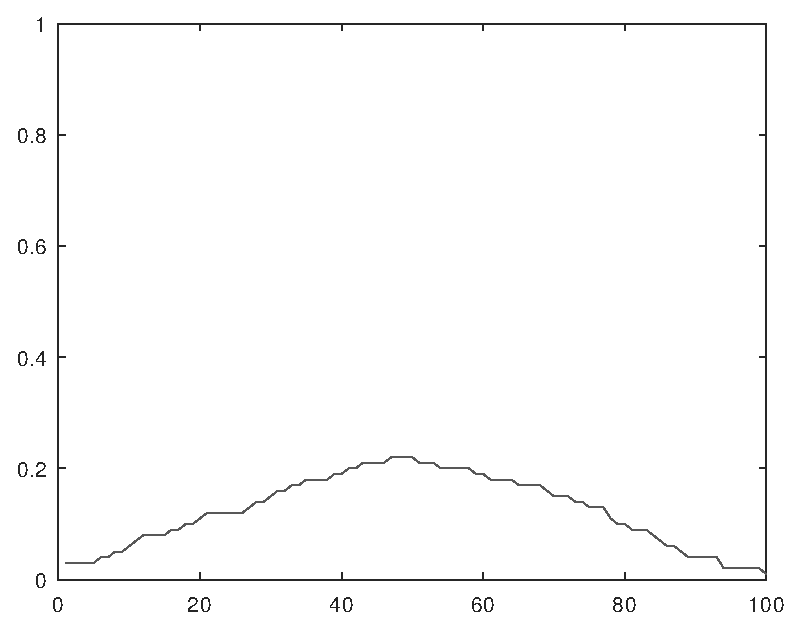
\includegraphics[width=.39\linewidth]{movement-rate-0.eps}
    \caption{Koeficient pohybu 0}
\end{figure}

\subsubsection{Experiment č. 2}
Experiment popisuje zmenu šírenia vírusu pri použití ochrany dýchacích ciest (rúška). V našom modeli predpokladáme, že 100\% obyvateľov používa chirurgické rúška a chirurgické rúško zadrží 75\% častíc.\cite{Masks}
Experiment prebiehal s hodnotou koeficientu pohybu rovnej 5.

\begin{figure}[h!]
    \center
    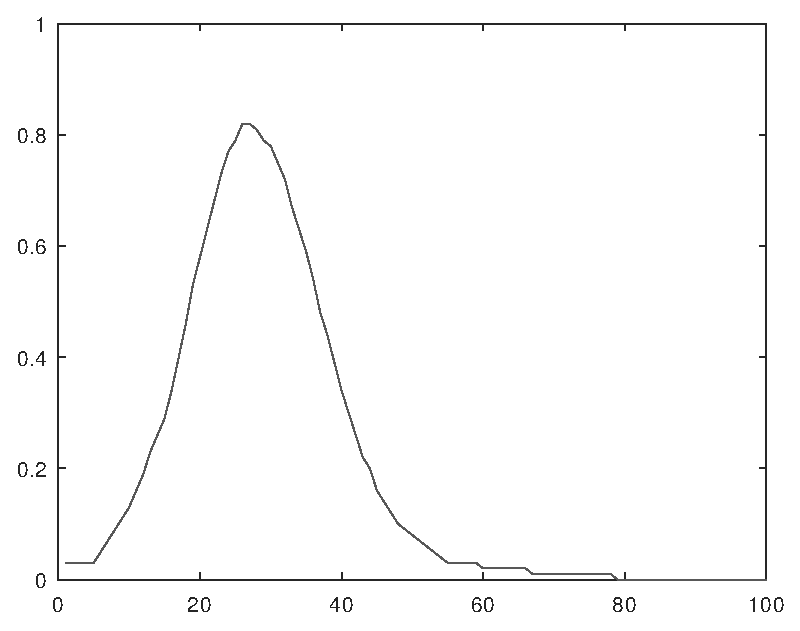
\includegraphics[width=.39\linewidth]{movement5transmission0,059.eps}
    \caption{0\% obyvateľov používa rúška}
\end{figure}

\begin{figure}[h!]
    \centering
    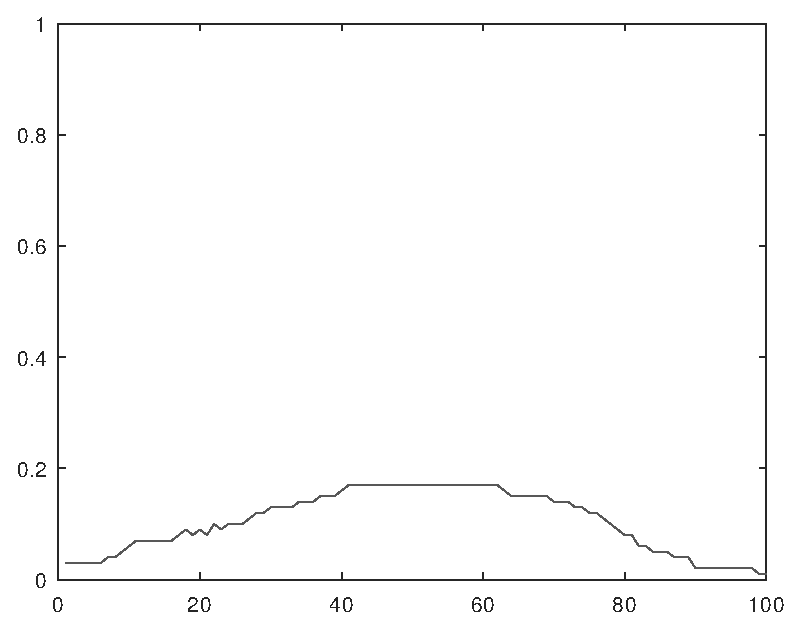
\includegraphics[width=.39\linewidth]{movement5transmission0,01475.eps}
    \caption{100\% obyvateľov používa rúška}
\end{figure}

\subsection{Závery experimentov}
Celkovo prebehli 2 experimenty: prvý s obmedzením pohybu a druhý s použitím masky. Model sa správal podľa očakávaní v oboch prípadoch.

\section{Zhrnutie simulačných experimentov a záver}
Z experimentov je jasné, že s menším koeficientom pohybu / použitím masky došlo k "splošteniu krivky" a teda výsledky sedia s ostatnými štúdiami. Je možné teda potvrdiť validitu modelu s dostatočnou dôveryhodnosťou. \cite{Experiment1}

\newpage
\renewcommand{\refname}{Referencie}
\bibliography{bibliography}

\end{document}
